\documentclass{article}
\usepackage{blindtext}
\usepackage{amsmath}
\usepackage{amssymb}
\usepackage{graphicx}
\usepackage[]{algorithm2e}
\usepackage[utf8]{inputenc}
\usepackage{listings}
\usepackage{color}
\usepackage{longtable}

\definecolor{dkgreen}{rgb}{0,0.6,0}
\definecolor{gray}{rgb}{0.5,0.5,0.5}
\definecolor{mauve}{rgb}{0.58,0,0.82}

\lstset{ %
    language=C,
    basicstyle={\small\ttfamily},% basic font setting
    keywordstyle=\color{blue},
    commentstyle=\color{dkgreen},
    stringstyle=\color{mauve},
    breakatwhitespace=true,
    tabsize=3
}

\newcommand\norm[1]{\left\lVert#1\right\rVert}

\begin{document}
\RestyleAlgo{boxruled}

\section{Introduction}

This read-me file describes a library written in C for fitting two-dimensional gaussian functions. To test this library, we have a Python script which interfaces with it using ctypes \cite{ctypes}. The Python script generates a random set of points in $\mathbb{R}^2$ over a region $x_{min}$, $x_{max}$, $y_{min}$ and $y_{max}$ with a uniform distribution. We use $N=10000$ and calculate the value $Z=f(X,Y)+\text{noise}$. Here, $f(X,Y)$ is a 2D Gaussian function:

\begin{equation}
f_{\overrightarrow{p}}(X,Y) = A\exp(-\frac{(X-\mu_x)^2}{2\sigma_x^2}-\frac{(Y-\mu_y)^2}{2\sigma_y^2}) + flr
\label{twoDGauss}
\end{equation}

The Python script also chooses the parameter vector of this function, \\$\overrightarrow{p}=[\mu_x, \mu_y, \sigma_x, \sigma_y, A, flr]^T$ at random. A successful test will retrive the parameters used to generate the dataset, within a margin of error. In addition, the Python script will graphically display the results of the fit in a plot. 

\section{Gauss-Newton method for iterative Least-Squares fitting} \label{sec_fit}

We use the Gauss-Newton method to fit a Gaussian function. This method can be summerized as follows:  

\begin{algorithm}[ht]
	\KwData{Column vectors of independent sample points $\overrightarrow{X}$ and $\overrightarrow{Y}$ and observations $\overrightarrow{Z}$ of length $N$}
	\KwResult{Find the parameter vector $\overrightarrow{p}$ which minimizes $\left|\overrightarrow{Z}-f_{\overrightarrow{p}}(\overrightarrow{X},\overrightarrow{Y})\right|$}
	First guess fit parameters $\overrightarrow{p}=\text{initial\_estimate}(\overrightarrow{X},\overrightarrow{Y},\overrightarrow{Z})$\;
	\While{True}{
		Evaluate the vector $\overrightarrow{r}=[r_1,r_2,..., r_N]^T$ with $r_n=Z_n-f_{p}(X_n,Y_n)$\;
		Evaluate jacobian $\mathbf{J}=\left[ \begin{array}{cccc}
		\frac{\partial r_1}{\partial p_1}, \frac{\partial r_1}{\partial p_2}, ..., \frac{\partial r_1}{\partial p_6} \\
		\frac{\partial r_2}{\partial p_1}, \frac{\partial r_2}{\partial p_2}, ..., \frac{\partial r_2}{\partial p_6} \\
		\vdots\\
		\frac{\partial r_N}{\partial p_1}, \frac{\partial r_N}{\partial p_2}, ..., \frac{\partial r_N}{\partial p_6} \\
		\end{array} \right]$\;
		Solve the equation $\mathbf{J}\Delta \overrightarrow{p} = \overrightarrow{r}$ for the vector $\Delta \overrightarrow{p}$\;
		Update the estimate of the parameters $\overrightarrow{p}=\overrightarrow{p}-\Delta \overrightarrow{p}$\;

		\If{$\left|\Delta \overrightarrow{p}\right|<0.001$}{
		exit loop\;
		}
	}
	
\end{algorithm}

We will denote the fitted parameter vector as $\overrightarrow{\tilde{p}}=[\tilde{\mu_x}, \tilde{\mu_y}, \tilde{\sigma_x}, \tilde{\sigma_y}, \tilde{A}, \tilde{flr}]^T$ in the rest of our document. 

\subsection{finding the initial estimates}

We estimate $flr$ and $A$ by simply finding the smallest and largest value of $Z$

\begin{align}
flr^* &= \min(Z) \\
A^* &= \max(Z)-\min(Z)
\end{align}

Symbols with an asterics mark $^*$ denote an initial estimate. The initial estimates for $\mu_x$ and $\mu_y$ are found by calculating the weighted center of mass of the $(X,Y)$ sample points with the weight factors given by $Z$ 

\begin{align}
\mu_x^* &= \frac{\sum\limits_{n=1}^N (Z_n-flr^*)X_n}{\sum\limits_{n=1}^N(Z_n-flr^*)}\\
\mu_y^* &= \frac{\sum\limits_{n=1}^N (Z_n-flr^*)Y_n}{\sum\limits_{n=1}^N(Z_n-flr^*)}
\end{align}

We find initial estimates for $\sigma_x$ and $\sigma_y$ by using the following property of the Gaussian function 

\begin{equation}
\int\limits_{-\infty}^{\infty}\int\limits_{-\infty}^{\infty}A\exp(-\frac{(X-\mu_x)^2}{2\sigma_x^2}-\frac{(Y-\mu_y)^2}{2\sigma_y^2})dxdy=2A\pi\sigma_x\sigma_y
\end{equation}

We approximate the double integral by a summation over $Z$ and find:

\begin{equation}
\Delta X\Delta Y\sum\limits_{n=1}^N(Z_n-flr^*) \cong 2A^*\pi\sigma_x\sigma_y
\end{equation}

Here $\Delta X = \frac{x_{max}-x_{min}}{\sqrt{N}}$ and $\Delta Y = \frac{y_{max}-y_{min}}{\sqrt{N}}$. By assuming $\sigma_x\cong\sigma_y$ we can find approximate values for $\sigma_x$ and $\sigma_y$ individually.


\begin{align}
\sigma_x^* &= \sqrt{\frac{\Delta X\Delta Y\sum\limits_{n=1}^N(Z_n-flr^*)}{2A^*\pi}}\\
\sigma_y^* &= \sigma_x^*
\end{align}

\section{Implementation and API}

The main function which does the fitting of a two-dimensional Gaussian function has the following prototype

\begin{center}
\begin{tabular}{|l|p{0.7\textwidth}|}
  \hline
  \textbf{prototype} & \begin{lstlisting} 
  int gaussian2DFit(double x[], 
					double y[], 
					double intensities[], 
					int dataSize, 
					double (*paramsArray)[])
  \end{lstlisting} \\
  \hline
  \multicolumn{2}{l}{\textbf{inputs}} \\
  \hline
  x & Array representing the x-coordinate of the points where we have sampled the observable \\
  \hline
  y & Array representing the y-coordinate of the points where we have sampled the observable \\
  \hline
  intensities & Array representing the values of the observables \\
  \hline
  dataSize & The length of the x, y and intensities arrays \\
  \hline
  \multicolumn{2}{l}{\textbf{outputs}} \\
  \hline
  paramsArray & The fitted parameters $[\mu_x, \mu_y, \sigma_x, \sigma_y, A, flr]$ \\
  \hline
  \multicolumn{2}{l}{\textbf{return value}} \\
  \hline
  EXIT\_FAIL (1) & If the fit has failed (e.g. the data is too noisy) \\
  \hline
  EXIT\_SUCCESS (0) & If the fit has succeeded \\
  \hline
\end{tabular}
\end{center}

In addition to the main fitting function, the library also exposes some underlying functions which are useful for general fitting purposes. 

\begin{center}
\begin{longtable}{|l|p{0.7\textwidth}|}
  \hline
  \textbf{prototype} & \begin{lstlisting} 
int gaussNewton(
matrix x, 
matrix y, 
matrix paramsInit,
int (*fitFunction)(matrix,matrix,matrix*),
double (*derivatives[])(matrix, matrix),
matrix *paramsFinal)
  \end{lstlisting} \\
  \hline
  \textbf{description} & This function uses the Gauss-Newton method to iteratively find the parameter vector $\overrightarrow{p}$ which minimizes $\left|y-f_{\overrightarrow{p}}(x)\right|$, where $f$ is the function we are fitting our data to. Note that this implementation requires that the derivatives of the fit function have known closed forms. \\
  \hline
  \multicolumn{2}{l}{\textbf{data structures}} \\
  \hline
  matrix & \begin{lstlisting} 
// In this code, matrix data is stored in 
// double arrays in a column wise fashion
// So if array A holds data of a 3-by-4 
// matrix, this should be interpreted as
//
//      A[0] A[1] A[2]  A[3]
//  A = A[4] A[5] A[6]  A[7]
//      A[8] A[9] A[10] A[11]
//
// Then, A.m = 3 and A.n = 4
typedef struct matrix
{
    double *data;
    int m;
    int n;
}matrix;
\end{lstlisting} \\
  \hline
  \multicolumn{2}{l}{\textbf{inputs}} \\
  \hline
  x & m-by-n Matrix holding the m independent variables in $\mathbb{R}^n$ space\\
  \hline
  y & m-by-1 Matrix holding the m dependent observables\\
  \hline
  paramsInit & p-by-1 matrix holding the initial estimates of p parameters \\
  \hline
  fitFunction & The first argument of this function is an m-by-n matrix holding the m independent variables in $\mathbb{R}^n$ space. The second argument is a p-by-1 matrix holding p parameters. The third argument is an output argument holding the result of the evaluation of the function at the locations of the independent variables, represented by an m-by-1 matrix. Memory for the matrix holding the evaluations will be allocated by the function being called\\
  \hline
  derivatives & An array of function pointers representing the derivatives of the fit function with respect to the parameter vector. The length of this function pointer array is equal to the number of parameters. The first argument of a derivative function is an m-by-n Matrix holding the m independent variables in $\mathbb{R}^n$ space. The second argument is a p-by-1 matrix holding p parameters. The functions will return a single double value\\
  \hline
  \multicolumn{2}{l}{\textbf{outputs}} \\
  \hline
  paramsFinal & The fitted parameters as an p-by-1 matrix \\
  \hline
  \multicolumn{2}{l}{\textbf{return value}} \\
  \hline
  EXIT\_FAIL (1) & If the fit has failed (e.g. the data is too noisy or maximum iterations reached) \\
  \hline
  EXIT\_SUCCESS (0) & If the fit has succeeded \\
  \hline
\end{longtable}
\end{center}

\begin{center}
\begin{longtable}{|l|p{0.7\textwidth}|}
  \hline
  \textbf{prototype} & \begin{lstlisting} 
int linearLeastSquares(
matrix X, 
matrix Y, 
matrix *b)
\end{lstlisting} \\
\hline
\textbf{description} & Find $\mathbf{b}$ for which $\norm{\mathbf{Xb}-\mathbf{Y}}^2$ is minimized. We use cholesky factorization to accomplish this\\
\hline
\multicolumn{2}{l}{\textbf{inputs}} \\
 \hline
x & $\mathbf{X}$ is a m-by-n matrix \\
\hline
y & $\mathbf{Y}$ is a m-by-o matrix \\
\hline
\multicolumn{2}{l}{\textbf{output}} \\
\hline
b & $\mathbf{b}$ is a n-by-o matrix \\
\hline
\multicolumn{2}{l}{\textbf{return value}} \\
\hline
EXIT\_FAIL & If the matrix $\mathbf{X}\mathbf{X}^T$ is not invertable \\
\hline
EXIT\_SUCCESS & If the fit has succeeded \\
\hline
\end{longtable} 
\end{center}

\section{Test Results}

As explained in the introduction, a Python script is used to test the library and visualize the results. We use ctypes to interface to the library, matplotlib for plotting and numpy for general math and statistical functions. 

An array $X$ of random values between the limits $x_{min}$, $x_{max}$ of length $N$ represents the x-coordinates where we sample function \ref{twoDGauss}. Similarly, an array $Y$ between $y_{min}$, $y_{max}$ of length $N$ represents the y-coordinates. We then contruct a Voronoi diagram based on these $X$ and $Y$ positions, where the interior color of the Voronoi cells are determined by the value of function \ref{twoDGauss} at that point. Figure \ref{fig_fit_part} illustrates this. 

\begin{figure}
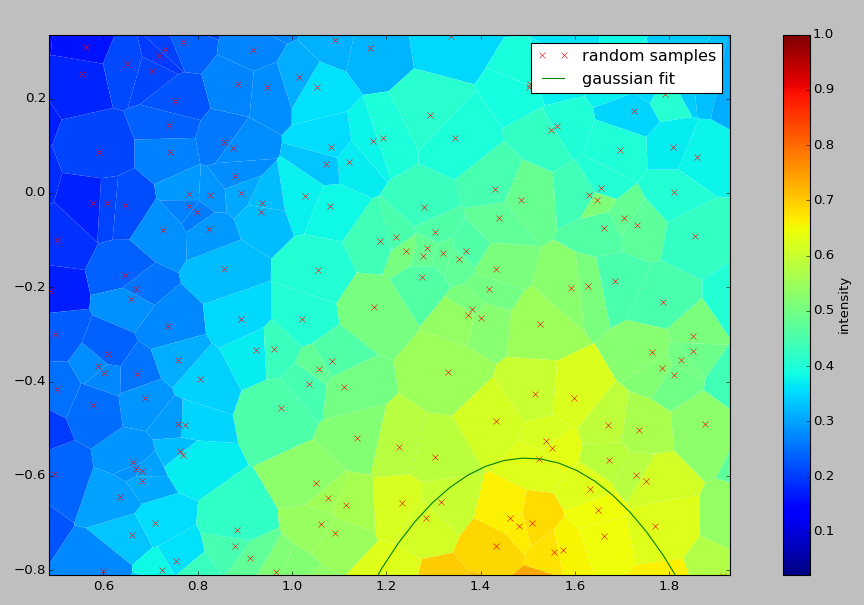
\includegraphics[width=1.0\textwidth]{randomSamples.png}
\caption{To visualize the fit results, we construct a Voronoi diagram based on the sample points $(X,Y)$, shown here as the red crosses. The interior color of the Voronoi cells are based on the value of the observation $Z$ at that point. The green solid line is an ellipse given by the implicit equation \ref{ellipse} }
\label{fig_fit_part}
\end{figure}

On this Voronoi diagram we superimpose a plot of an ellipse given by the implicit equation;

\begin{equation}
\left(\frac{x-\tilde{\mu_x}}{\tilde{\sigma_x}}\right)^2+\left(\frac{y-\tilde{\mu_y}}{\tilde{\sigma_y}}\right)^2=1
\label{ellipse}
\end{equation}

To reiterate, $\tilde{\mu_x}$, $\tilde{\mu_y}$, $\tilde{\sigma_x}$ and $\tilde{\sigma_y}$ are estimates of the parameters used to generated the dataset $(X,Y,Z)$ by applying the least squares fit as outlined in section \ref{sec_fit}

The results of a complete fit are shown in figure \ref{fig_fit}. 

\begin{figure}
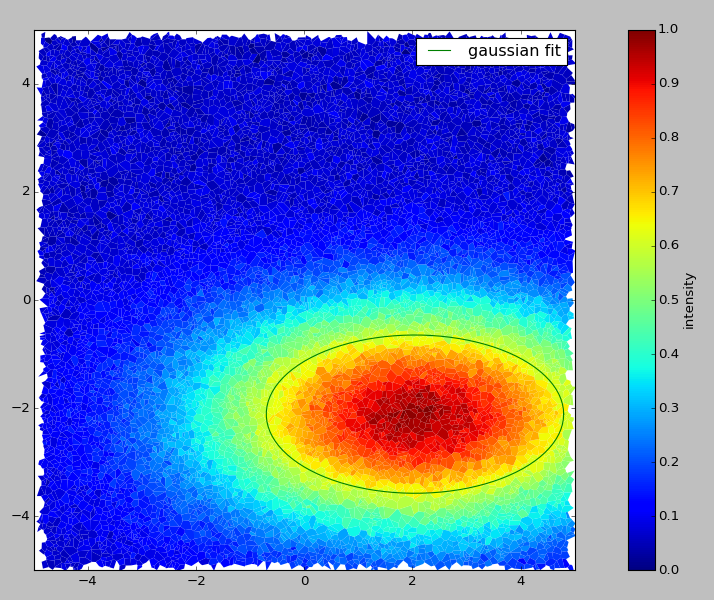
\includegraphics[width=1.0\textwidth]{randomSamples_whole.png}
\caption{Here we see the results of our fitting libarary on the entire dataset}
\label{fig_fit}
\end{figure}

\bibliographystyle{plain}
\bibliography{krissp-ctypes} 

\end{document}
